% --------------------------------------------------------------------------
% Template for ICAD-2024 paper; to be used with:
%          icad2024.sty  - ICAD 2024 LaTeX style file, and 2024
%          IEEEbtran.bst - IEEE bibliography style file.
%
% --------------------------------------------------------------------------
\UseRawInputEncoding
\documentclass[a4paper,10pt,oneside]{article}
\usepackage[utf8]{inputenc}
\usepackage{icad2024,amsmath,epsfig,times,url,hyperref}
\usepackage[T1]{fontenc}
\usepackage{graphicx}
\graphicspath{ {./images/} }

% Example definitions.
% --------------------


% Title.
% --------------------
\title{K-Nearest Neighbours Laboratory}

% *** IMPORTANT ***
% *** PLEASE LEAVE AUTHOR INFORMATION BLANK UNTIL FINAL CAMERA-READY SUBMISSION *** 

% IF ONE AUTHOR
%\name{Jyri Huopaniemi} 
%\address{Nokia Research Center \\ 
%Speech and Audio Systems Laboratory \\ 
%P.O.Box 407, FIN-00045 Nokia Group, Finland \\ 
%{\tt jyri.huopaniemi@nokia.com}} 
%

% IF TWO AUTHORS
\twoauthors
{Gabriele Francesco Berruti} {University of Genoa \\ Via Roma 37/6 \\ Genova, Italy  \\ {\tt gabriele.berruti@unige.edu}}
{Ibrahim Altufayli} {University of Genoa \\ Via Roma 37/6 \\ Genova, Italy  \\ {\tt ibrahim.altufayli@unige.edu}}

\begin{document}
\maketitle

\begin{abstract}
This report centers on the k-NN algorithm due to its intuitive nature and 
practical effectiveness. The lab objective is to construct a KNN classifier
and train it on synthetic 2D data for binary classification, incorporating noise 
to assess its impact on performance. 
The lab entails visualizing how the classifier separates data in 2D space and computing misclassification rates. The evaluation section focuses on comparing noisy and clean datasets, exploring varying noise levels and adjusting the number of neighbors (k).
The experiments showed something important: 
When there's a lot of noise in the data, we need to use a higher 'k' 
value to estimate a more complicated decision boundary.
But when the data is cleaner, we can use a smaller 'k' value to estimate a 
simpler function.
This means the k-NN method can adjust to different types of data, which is 
really useful in practical situations where data might not always be perfect.
\end{abstract}


\section{Introduction}
\label{sec:intro}

Classification is a fundamental task in machine learning that involves sorting 
data into categories. It's like teaching a computer to recognize patterns and 
decide which group new data belongs to. 
This process is essential in various applications, such as spam detection, 
image recognition, and medical diagnosis.
Several methods have been developed for classification, each with its own 
strengths and weaknesses. Simple methods like Decision Trees, Naive Bayes, 
and Logistic Regression are widely used due to their ease of implementation 
and interpretability. However, among these, the k-Nearest Neighbors (k-NN) 
algorithm stands out for its simplicity and effectiveness.
k-NN is a type of instance-based learning, where the algorithm makes decisions 
based on the closest data points in the training set. When a new data point needs
to be classified, k-NN looks at the 'k' nearest neighbors and assigns the most
common category among them to the new point. This approach makes k-NN intuitive
and easy to understand.
In this report, we focus on k-NN for its straightforward mechanism and practical
effectiveness. 
The goal of this lab is to build a KNN classifier and train it on a synthetic
 2D dataset for binary classification that we create. We will then add noise to
the data to see how it impacts the KNN's performance, making the task more challenging. The lab includes visualizing how the classifier separates the data in 2D space and calculating the percentage of incorrectly classified points out of the total samples.
After setting everything up, we will run experiments to compare how well the classifier works with both clean and noisy data, by changing the amount of noise and the value of 'k'.

\section{ Algorithms and Methods }
\label{sec:format}
In this section we will describe the different Algorithms and Methods have been 
implement or used in the lab.

\subsection{ Dataset generation for binary classification }
\label{ssec:subhead}
We start by generating a training set for binary classification problems. 
This involves creating random 2D points on a plane and assigning them binary 
labels based on their position relative to a linear separator.
The function linearBinaryClass takes a sample size n, lower and upper bounds 
"low D", "high D" for the domain of the samples, and the linear function 
parameters m, q to generate a binary classification dataset, 
returning X(consists of 2-dimensional samples) and Y
(consists of 1-dimensional binary labels).

\subsection{ Computing the distance between input points }
\label{ssec:subhead}
To build the KNN estimator, we need to use a distance function. 
We implemented a function that calculates the Euclidean distance
between two points in 2D space.

\subsection{ Adding noise to the samples }
\label{ssec:subhead}
To make the task harder, we may want to perturb the labels with some noise.
In our case, we have binary labels and a common way of adding noise is to 
flip the value of a small percentage of the labels. 
For example, if a label was a+b it will become a-b.

\subsection{ The KNN classifier }
\label{ssec:subhead}
It takes four parameters: Xtr (training data inputs), Ytr (training data labels), k (number of nearest neighbors to consider), and Xte (test data inputs).
First, it checks if the labels in Ytr are either +1 or -1, raising an exception if not. It then adjusts k if it exceeds the number of training samples.
The function initializes an array Ypred to store the predicted labels for the test data points.
Next, it calculates the Euclidean distances between each test sample in Xte and all training samples in Xtr.
For each test sample, it retrieves the distances to all training samples, sorts them, and selects the indices of the k nearest neighbors. It then computes the average label of these nearest neighbors and assigns the sign of this average as the predicted label for the test sample.
Finally, the function returns the array Ypred containing the predicted labels for the test data points.

\subsection{ Visualizing the separating function}
\label{ssec:subhead}
visualizes the separating function on the training set, which is the function estimated by the classification algorithm to discriminate between classes. It takes three parameters: Xtr (the matrix of training set inputs), Ytr (the array of training set labels), and k (the number of neighbors to consider).
It interpolates the predicted labels (Ypred) to create a continuous representation of the separating function, then plots the contour lines indicating the decision boundaries.

\subsection{ Evaluating the goodness of a classifier}
\label{ssec:subhead}
To evaluate how good is the classification function estimated by the KNN, 
we compare the predicted binary labels and expected (true) ones.
It then counts the number of elements where the predicted label is not equal 
to the true label, to claculate the error rate.
This error rate represents the proportion of misclassified samples out 
of all samples in the dataset.

\section{ Experimental analysis }
\label{sec:typestyle}

\subsection{ Experiment with not-noisy data }
\label{ssec:not-noisy}

In the first section we will first evaluate the behavior of the KNN classifier 
on the training set and the test set in the case in which the creation of thetwo datasets will 
take place without noise. 
In particular, in this phase we specify the parameters relating 
to the number of samples to be generated, the lower and upper bounds for 
the domain of the samples and the parameters relating to the linear function 
(1) which will allow the data to be generated . 
At the end of this procedure we will obtain 2-dimensional samples (X) associated 
with 1-dimensional binary labels (Y), where the Y labels represents the real 
values linked to the training set .
One of the metrics that we will adopt in this section involves the calculation 
of the error between the predictions made by the model trained on the training 
set and the test set (or the training set itself). 
The first experiments we carry out in this phase is to evaluate the classifier 
on the training set with a parameter k equal to 1. 
So after training the model on the training set we evaluate it on the same set.
As you can imagine, the error obtained is equal to zero since the values in the 
two set are literally the same.
In the second experiment, similarly to what we did previously, we carry out a 
comparison between two sets where however they present different values 
(even if the generation is still described by a linear function) . 
The results obtained by using and comparing the training set and the test 
set with k=1 allow us to obtain an error of 0.03, which means that 3 percent 
of the predictions made on the test set do not correspond to the real values.
This behavior is due to the fact that using such a low parameter k does not 
allow us to extrapolate the form of the function since we restrict the search to
a single (nearby) element and not to a series as we will see later.

\begin{figure}[h]
  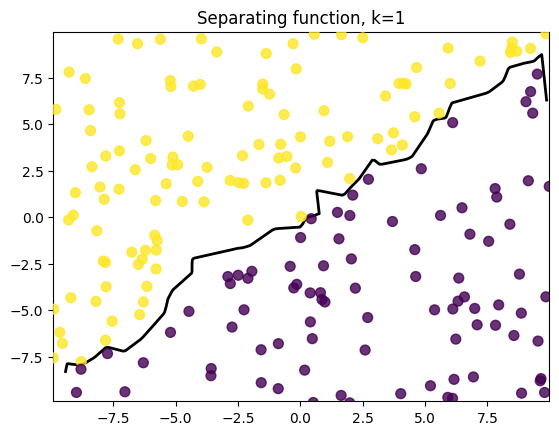
\includegraphics[width=8cm]{first_experiment.png}
  \caption{Example of a non-noisy dataset}
\end{figure}

\subsection{ Experiment with Noisy data and different K }
\label{ssec:noisy}
This section will deal (as can be understood from the title) with the comparison 
between two sets (training and set similarly to before) in which, however, 
the generation of data will be disturbed by random noise which does not 
allow the data to be distributed according to only a linear function with 
different parameters.
Specifically, randomness mainly refers to which of the two labels to associate the pair of 
values.
The quantity of pairs (in percentage) at which the labels will be modified is 
determined by the parameter P while the quantity of neighbors to take into
consideration is always managed by k. 
In the first experiment of this section, a value of 10 is associated with 
the parameter P (which indicates changing 10 percent of the labels) while k 
remains equal to 1 (from the previous experiment).
From this experiment we can see how the error obtained on the training set continues 
to remain equal to zero since the algorithm will once again compare two identical sets.
The situation however varies when we feed the test set to the algorithm, in this case the 
calculated error is 0.19, which indicates that approximately 20 percent of the predicted 
labels do not reflect the real labels.
Making a comparison with the experiment without noise, we note that the error increases 
considerably . 
By fixing the parameters decided previously and modifying exclusively the value of k 
we can notice that the results vary considerably. 
For example, using a K equal to 5, and therefore evaluating the classifier on the
training set itself, we notice an unusual behavior, i.e. the error 
on the predictions is higher than that where k was equal to 1. 
Varying from 0 to 0.115 .
This is because observing a larger spectrum of nearby pairs can lead to a
prediction that is different from the actual label.
Furthermore, it is useful to note that the percentage error value is comparable 
to the value of labels that are "flipped", this is because the "noisy" pairs 
will most likely be "immersed" in a neighborhood composed of pairs belonging
to the other label .
The situation is reversed when we evaluate the noisy data on the test set. 
In this case the error decreases compared to the previous case, varying from 0.19 to 0.145.
This is due to the fact that, even if the data are noisy, the values that are along or 
near the separation function will have a better spectrum of elements to compare with
will be able to determine their label in a more coherent way while for the elements 
in the test sets (as in the training set) that are surrounded only by labels that differ 
from the real one there is no possibility that they will be associated correctly.
Finally, the last experiment involves the use of a k equal to 10. 
This value allows us to increase the number of neighboring pairs with which it
is possible to compare. In this specific situation the choice of the aforementioned 
parameter allows the classifier to obtain a slightly worse result than the error 
relating to the k equal 5, since the error between the predicted value and the real 
one varies from 0.115 to 0.135 while the calculation of the error on the test part 
goes from 0.145 to 0.11.
These results depend a lot on the random generation of the data but it can still 
be noted that a smaller k causes the classifier to fall in love with the data 
(overfitting the training set) while increasing k in general tends to generalize 
more because it searches in a wider area . \\
\begin{figure}[h]
  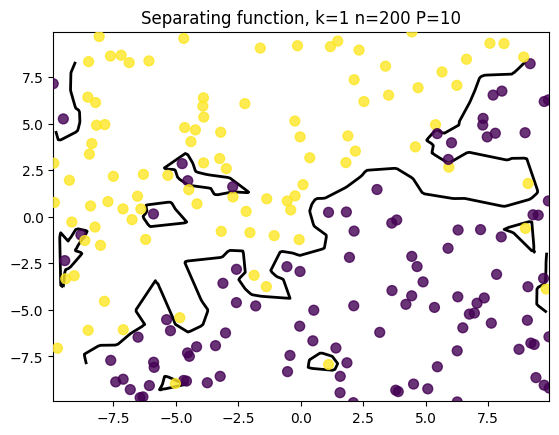
\includegraphics[width=8cm]{second_experiment.png}
  \caption{ Example of a noisy dataset }
\end{figure}

\section{ Conclusions }
\label{sec:majhead}

The experiments clearly demonstrate that the choice of 'k' in the k-NN 
algorithm depends on the level of noise in the data. When dealing with 
noisy data, a higher 'k' is necessary to build a more complex decision 
boundary that can effectively separate signal from noise. Conversely, 
in cleaner datasets, lower 'k' values are enough to capture the underlying 
patterns in the data without being overly influenced by noise. 
This showed the importance of tailoring the choice of 'k' to the specific 
characteristics of the dataset, optimizing the algorithm's performance 
for different levels of data quality.\\

\section{Equations}
\label{sec:equations}

Equations of the linear function : (\ref{eqn:wave_equation})
\cite{eWilliams1999},

\begin{equation}
  \label{eqn:wave_equation}
     f( x ) = m (x) + q 
\end{equation}
where $f(x)$ is the function that 
allows us to sub-divide data ( by associating a label ) based on the 
parameters m and q which represents the angular 
coefficient and the coefficient q is a known term .



\bibliographystyle{IEEEtran}
\bibliography{refs2024}

\end{document}
